% Options for packages loaded elsewhere
\PassOptionsToPackage{unicode}{hyperref}
\PassOptionsToPackage{hyphens}{url}
\PassOptionsToPackage{dvipsnames,svgnames,x11names}{xcolor}
%
\documentclass[
  letterpaper,
  DIV=11,
  numbers=noendperiod]{scrartcl}

\usepackage{amsmath,amssymb}
\usepackage{iftex}
\ifPDFTeX
  \usepackage[T1]{fontenc}
  \usepackage[utf8]{inputenc}
  \usepackage{textcomp} % provide euro and other symbols
\else % if luatex or xetex
  \usepackage{unicode-math}
  \defaultfontfeatures{Scale=MatchLowercase}
  \defaultfontfeatures[\rmfamily]{Ligatures=TeX,Scale=1}
\fi
\usepackage{lmodern}
\ifPDFTeX\else  
    % xetex/luatex font selection
\fi
% Use upquote if available, for straight quotes in verbatim environments
\IfFileExists{upquote.sty}{\usepackage{upquote}}{}
\IfFileExists{microtype.sty}{% use microtype if available
  \usepackage[]{microtype}
  \UseMicrotypeSet[protrusion]{basicmath} % disable protrusion for tt fonts
}{}
\makeatletter
\@ifundefined{KOMAClassName}{% if non-KOMA class
  \IfFileExists{parskip.sty}{%
    \usepackage{parskip}
  }{% else
    \setlength{\parindent}{0pt}
    \setlength{\parskip}{6pt plus 2pt minus 1pt}}
}{% if KOMA class
  \KOMAoptions{parskip=half}}
\makeatother
\usepackage{xcolor}
\setlength{\emergencystretch}{3em} % prevent overfull lines
\setcounter{secnumdepth}{5}
% Make \paragraph and \subparagraph free-standing
\ifx\paragraph\undefined\else
  \let\oldparagraph\paragraph
  \renewcommand{\paragraph}[1]{\oldparagraph{#1}\mbox{}}
\fi
\ifx\subparagraph\undefined\else
  \let\oldsubparagraph\subparagraph
  \renewcommand{\subparagraph}[1]{\oldsubparagraph{#1}\mbox{}}
\fi

\usepackage{color}
\usepackage{fancyvrb}
\newcommand{\VerbBar}{|}
\newcommand{\VERB}{\Verb[commandchars=\\\{\}]}
\DefineVerbatimEnvironment{Highlighting}{Verbatim}{commandchars=\\\{\}}
% Add ',fontsize=\small' for more characters per line
\usepackage{framed}
\definecolor{shadecolor}{RGB}{241,243,245}
\newenvironment{Shaded}{\begin{snugshade}}{\end{snugshade}}
\newcommand{\AlertTok}[1]{\textcolor[rgb]{0.68,0.00,0.00}{#1}}
\newcommand{\AnnotationTok}[1]{\textcolor[rgb]{0.37,0.37,0.37}{#1}}
\newcommand{\AttributeTok}[1]{\textcolor[rgb]{0.40,0.45,0.13}{#1}}
\newcommand{\BaseNTok}[1]{\textcolor[rgb]{0.68,0.00,0.00}{#1}}
\newcommand{\BuiltInTok}[1]{\textcolor[rgb]{0.00,0.23,0.31}{#1}}
\newcommand{\CharTok}[1]{\textcolor[rgb]{0.13,0.47,0.30}{#1}}
\newcommand{\CommentTok}[1]{\textcolor[rgb]{0.37,0.37,0.37}{#1}}
\newcommand{\CommentVarTok}[1]{\textcolor[rgb]{0.37,0.37,0.37}{\textit{#1}}}
\newcommand{\ConstantTok}[1]{\textcolor[rgb]{0.56,0.35,0.01}{#1}}
\newcommand{\ControlFlowTok}[1]{\textcolor[rgb]{0.00,0.23,0.31}{#1}}
\newcommand{\DataTypeTok}[1]{\textcolor[rgb]{0.68,0.00,0.00}{#1}}
\newcommand{\DecValTok}[1]{\textcolor[rgb]{0.68,0.00,0.00}{#1}}
\newcommand{\DocumentationTok}[1]{\textcolor[rgb]{0.37,0.37,0.37}{\textit{#1}}}
\newcommand{\ErrorTok}[1]{\textcolor[rgb]{0.68,0.00,0.00}{#1}}
\newcommand{\ExtensionTok}[1]{\textcolor[rgb]{0.00,0.23,0.31}{#1}}
\newcommand{\FloatTok}[1]{\textcolor[rgb]{0.68,0.00,0.00}{#1}}
\newcommand{\FunctionTok}[1]{\textcolor[rgb]{0.28,0.35,0.67}{#1}}
\newcommand{\ImportTok}[1]{\textcolor[rgb]{0.00,0.46,0.62}{#1}}
\newcommand{\InformationTok}[1]{\textcolor[rgb]{0.37,0.37,0.37}{#1}}
\newcommand{\KeywordTok}[1]{\textcolor[rgb]{0.00,0.23,0.31}{#1}}
\newcommand{\NormalTok}[1]{\textcolor[rgb]{0.00,0.23,0.31}{#1}}
\newcommand{\OperatorTok}[1]{\textcolor[rgb]{0.37,0.37,0.37}{#1}}
\newcommand{\OtherTok}[1]{\textcolor[rgb]{0.00,0.23,0.31}{#1}}
\newcommand{\PreprocessorTok}[1]{\textcolor[rgb]{0.68,0.00,0.00}{#1}}
\newcommand{\RegionMarkerTok}[1]{\textcolor[rgb]{0.00,0.23,0.31}{#1}}
\newcommand{\SpecialCharTok}[1]{\textcolor[rgb]{0.37,0.37,0.37}{#1}}
\newcommand{\SpecialStringTok}[1]{\textcolor[rgb]{0.13,0.47,0.30}{#1}}
\newcommand{\StringTok}[1]{\textcolor[rgb]{0.13,0.47,0.30}{#1}}
\newcommand{\VariableTok}[1]{\textcolor[rgb]{0.07,0.07,0.07}{#1}}
\newcommand{\VerbatimStringTok}[1]{\textcolor[rgb]{0.13,0.47,0.30}{#1}}
\newcommand{\WarningTok}[1]{\textcolor[rgb]{0.37,0.37,0.37}{\textit{#1}}}

\providecommand{\tightlist}{%
  \setlength{\itemsep}{0pt}\setlength{\parskip}{0pt}}\usepackage{longtable,booktabs,array}
\usepackage{calc} % for calculating minipage widths
% Correct order of tables after \paragraph or \subparagraph
\usepackage{etoolbox}
\makeatletter
\patchcmd\longtable{\par}{\if@noskipsec\mbox{}\fi\par}{}{}
\makeatother
% Allow footnotes in longtable head/foot
\IfFileExists{footnotehyper.sty}{\usepackage{footnotehyper}}{\usepackage{footnote}}
\makesavenoteenv{longtable}
\usepackage{graphicx}
\makeatletter
\def\maxwidth{\ifdim\Gin@nat@width>\linewidth\linewidth\else\Gin@nat@width\fi}
\def\maxheight{\ifdim\Gin@nat@height>\textheight\textheight\else\Gin@nat@height\fi}
\makeatother
% Scale images if necessary, so that they will not overflow the page
% margins by default, and it is still possible to overwrite the defaults
% using explicit options in \includegraphics[width, height, ...]{}
\setkeys{Gin}{width=\maxwidth,height=\maxheight,keepaspectratio}
% Set default figure placement to htbp
\makeatletter
\def\fps@figure{htbp}
\makeatother

\KOMAoption{captions}{tableheading}
\makeatletter
\makeatother
\makeatletter
\makeatother
\makeatletter
\@ifpackageloaded{caption}{}{\usepackage{caption}}
\AtBeginDocument{%
\ifdefined\contentsname
  \renewcommand*\contentsname{Table of contents}
\else
  \newcommand\contentsname{Table of contents}
\fi
\ifdefined\listfigurename
  \renewcommand*\listfigurename{List of Figures}
\else
  \newcommand\listfigurename{List of Figures}
\fi
\ifdefined\listtablename
  \renewcommand*\listtablename{List of Tables}
\else
  \newcommand\listtablename{List of Tables}
\fi
\ifdefined\figurename
  \renewcommand*\figurename{Figure}
\else
  \newcommand\figurename{Figure}
\fi
\ifdefined\tablename
  \renewcommand*\tablename{Table}
\else
  \newcommand\tablename{Table}
\fi
}
\@ifpackageloaded{float}{}{\usepackage{float}}
\floatstyle{ruled}
\@ifundefined{c@chapter}{\newfloat{codelisting}{h}{lop}}{\newfloat{codelisting}{h}{lop}[chapter]}
\floatname{codelisting}{Listing}
\newcommand*\listoflistings{\listof{codelisting}{List of Listings}}
\makeatother
\makeatletter
\@ifpackageloaded{caption}{}{\usepackage{caption}}
\@ifpackageloaded{subcaption}{}{\usepackage{subcaption}}
\makeatother
\makeatletter
\@ifpackageloaded{tcolorbox}{}{\usepackage[skins,breakable]{tcolorbox}}
\makeatother
\makeatletter
\@ifundefined{shadecolor}{\definecolor{shadecolor}{rgb}{.97, .97, .97}}
\makeatother
\makeatletter
\makeatother
\makeatletter
\makeatother
\ifLuaTeX
  \usepackage{selnolig}  % disable illegal ligatures
\fi
\IfFileExists{bookmark.sty}{\usepackage{bookmark}}{\usepackage{hyperref}}
\IfFileExists{xurl.sty}{\usepackage{xurl}}{} % add URL line breaks if available
\urlstyle{same} % disable monospaced font for URLs
\hypersetup{
  pdftitle={Multiple panels and multiple graphs},
  pdfauthor={Justin Baumann},
  colorlinks=true,
  linkcolor={blue},
  filecolor={Maroon},
  citecolor={Blue},
  urlcolor={Blue},
  pdfcreator={LaTeX via pandoc}}

\title{Multiple panels and multiple graphs}
\author{Justin Baumann}
\date{}

\begin{document}
\maketitle
\ifdefined\Shaded\renewenvironment{Shaded}{\begin{tcolorbox}[boxrule=0pt, frame hidden, sharp corners, enhanced, interior hidden, borderline west={3pt}{0pt}{shadecolor}, breakable]}{\end{tcolorbox}}\fi

\renewcommand*\contentsname{Table of contents}
{
\hypersetup{linkcolor=}
\setcounter{tocdepth}{3}
\tableofcontents
}
Often in science we are interested in comparing several graphs at once
or looking at 3 or 4 variables at a time. This means we may want to have
multi-panel graphs or multiple graphs on the same page. While it is
common to produce graphs in R and combine them into ``final'' manuscript
ready version in other programs, such as Adobe Illustrator or Inkscape
(a free alternative to Illustrator), producing manuscript quality
figures in R is possible! In fact, it is only getting easier, thanks to
some new packages (like patchwork). Below I will show you how to make
multipanel figures (aka facets) and how to put many figures on one page
(using the patchwork package-- the easiest of the many options for doing
this).

\begin{Shaded}
\begin{Highlighting}[]
\CommentTok{\#Load packages}
\FunctionTok{library}\NormalTok{(tidyverse)}
\end{Highlighting}
\end{Shaded}

\begin{verbatim}
-- Attaching packages --------------------------------------- tidyverse 1.3.2 --
v ggplot2 3.4.0      v purrr   1.0.0 
v tibble  3.1.8      v dplyr   1.0.10
v tidyr   1.2.1      v stringr 1.5.0 
v readr   2.1.3      v forcats 0.5.2 
-- Conflicts ------------------------------------------ tidyverse_conflicts() --
x dplyr::filter() masks stats::filter()
x dplyr::lag()    masks stats::lag()
\end{verbatim}

\begin{Shaded}
\begin{Highlighting}[]
\FunctionTok{library}\NormalTok{(ggsci) }\CommentTok{\#for easy color scales}
\FunctionTok{library}\NormalTok{(patchwork) }\CommentTok{\#to make multi{-}panel plots }
\FunctionTok{library}\NormalTok{(palmerpenguins) }\CommentTok{\# our fave penguin friends :)}
\end{Highlighting}
\end{Shaded}

\hypertarget{facets}{%
\subsection{\texorpdfstring{\textbf{facets}}{facets}}\label{facets}}

Facets allow us to produce multiple graph panels with one ggplot code.
We can separate out a variable for easier viewing or even create a grid
of graphs using multiple variables.

facet\_wrap() allows us to make multiple panels. The panels are aligned
in columns and rows. We need to use `\textasciitilde{}' in our
facet\_wrap code. The `\textasciitilde{}' essentially means ``by''

\begin{Shaded}
\begin{Highlighting}[]
\FunctionTok{ggplot}\NormalTok{(}\AttributeTok{data=}\NormalTok{penguins, }\FunctionTok{aes}\NormalTok{(}\AttributeTok{x=}\NormalTok{island, }\AttributeTok{y=}\NormalTok{ bill\_length\_mm, }\AttributeTok{fill=}\NormalTok{species)) }\SpecialCharTok{+}
  \FunctionTok{geom\_boxplot}\NormalTok{()}\SpecialCharTok{+}
  \FunctionTok{facet\_wrap}\NormalTok{(}\SpecialCharTok{\textasciitilde{}}\NormalTok{island)}\SpecialCharTok{+}
  \FunctionTok{scale\_color\_aaas}\NormalTok{()}\SpecialCharTok{+}
  \FunctionTok{theme\_classic}\NormalTok{()}
\end{Highlighting}
\end{Shaded}

\begin{verbatim}
Warning: Removed 2 rows containing non-finite values (`stat_boxplot()`).
\end{verbatim}

\begin{figure}[H]

{\centering 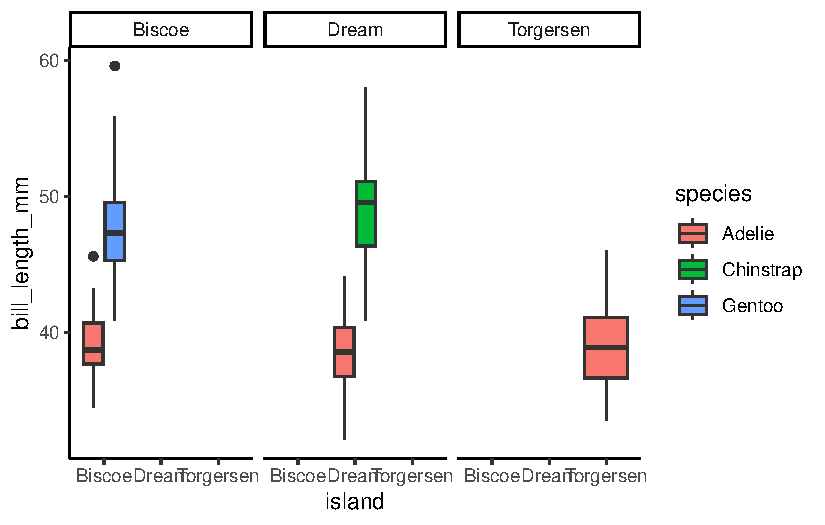
\includegraphics{facets_files/figure-pdf/unnamed-chunk-2-1.pdf}

}

\end{figure}

We can specify the number of columns and rows we want to built the
panels how we like them

\begin{Shaded}
\begin{Highlighting}[]
\FunctionTok{ggplot}\NormalTok{(}\AttributeTok{data=}\NormalTok{penguins, }\FunctionTok{aes}\NormalTok{(}\AttributeTok{x=}\NormalTok{year, }\AttributeTok{y=}\NormalTok{ bill\_length\_mm, }\AttributeTok{fill=}\NormalTok{species)) }\SpecialCharTok{+}
  \FunctionTok{geom\_boxplot}\NormalTok{()}\SpecialCharTok{+}
  \FunctionTok{facet\_wrap}\NormalTok{(}\SpecialCharTok{\textasciitilde{}}\NormalTok{island, }\AttributeTok{ncol=}\DecValTok{2}\NormalTok{)}\SpecialCharTok{+} \CommentTok{\#2 columns }
  \FunctionTok{scale\_color\_aaas}\NormalTok{()}\SpecialCharTok{+}
  \FunctionTok{theme\_classic}\NormalTok{()}
\end{Highlighting}
\end{Shaded}

\begin{verbatim}
Warning: Removed 2 rows containing non-finite values (`stat_boxplot()`).
\end{verbatim}

\begin{figure}[H]

{\centering 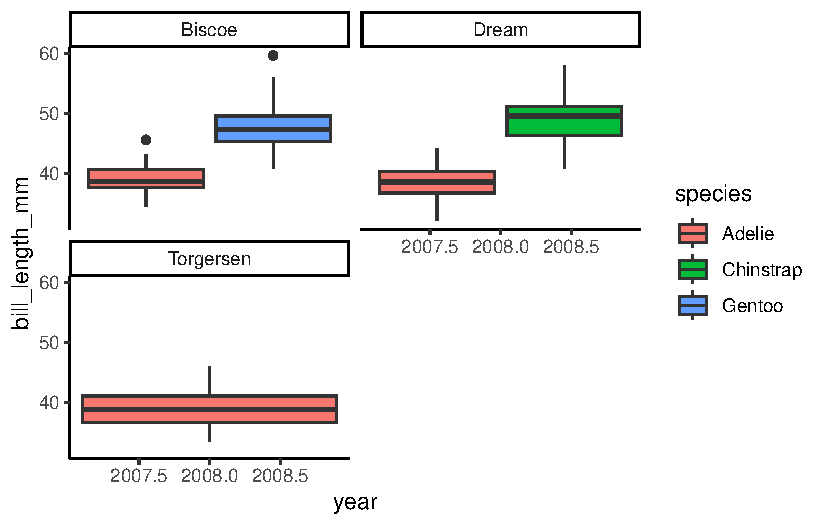
\includegraphics{facets_files/figure-pdf/unnamed-chunk-3-1.pdf}

}

\end{figure}

\begin{Shaded}
\begin{Highlighting}[]
\FunctionTok{ggplot}\NormalTok{(}\AttributeTok{data=}\NormalTok{penguins, }\FunctionTok{aes}\NormalTok{(}\AttributeTok{x=}\NormalTok{year, }\AttributeTok{y=}\NormalTok{ bill\_length\_mm, }\AttributeTok{fill=}\NormalTok{species)) }\SpecialCharTok{+}
  \FunctionTok{geom\_boxplot}\NormalTok{()}\SpecialCharTok{+}
  \FunctionTok{facet\_wrap}\NormalTok{(}\SpecialCharTok{\textasciitilde{}}\NormalTok{island, }\AttributeTok{nrow=}\DecValTok{3}\NormalTok{)}\SpecialCharTok{+} \CommentTok{\#3 rows}
  \FunctionTok{scale\_color\_aaas}\NormalTok{()}\SpecialCharTok{+}
  \FunctionTok{theme\_classic}\NormalTok{()}
\end{Highlighting}
\end{Shaded}

\begin{verbatim}
Warning: Removed 2 rows containing non-finite values (`stat_boxplot()`).
\end{verbatim}

\begin{figure}[H]

{\centering 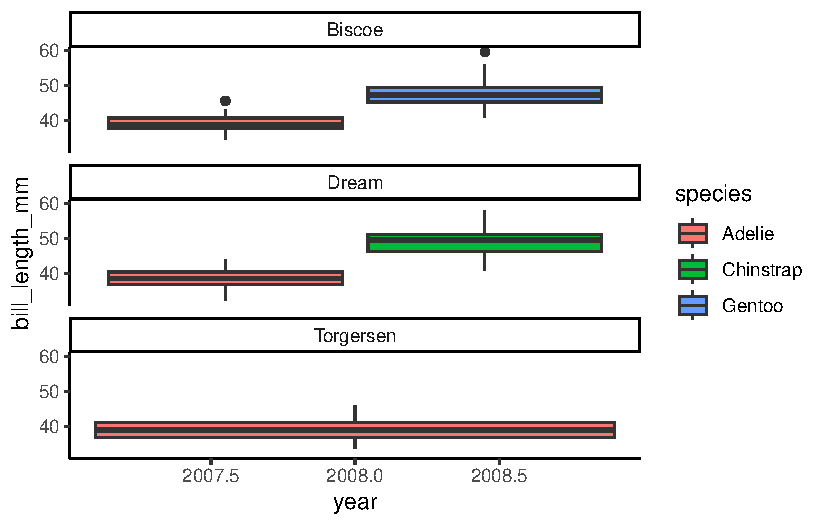
\includegraphics{facets_files/figure-pdf/unnamed-chunk-4-1.pdf}

}

\end{figure}

We can even use a formula for building our facets if we'd like!

\begin{Shaded}
\begin{Highlighting}[]
\FunctionTok{ggplot}\NormalTok{(}\AttributeTok{data=}\NormalTok{penguins, }\FunctionTok{aes}\NormalTok{(}\AttributeTok{x=}\NormalTok{island, }\AttributeTok{y=}\NormalTok{ bill\_length\_mm, }\AttributeTok{fill=}\NormalTok{species)) }\SpecialCharTok{+}
  \FunctionTok{geom\_boxplot}\NormalTok{()}\SpecialCharTok{+}
  \FunctionTok{facet\_wrap}\NormalTok{(}\SpecialCharTok{\textasciitilde{}}\NormalTok{species}\SpecialCharTok{+}\NormalTok{year)}\SpecialCharTok{+}
  \FunctionTok{scale\_color\_aaas}\NormalTok{()}\SpecialCharTok{+}
  \FunctionTok{theme\_classic}\NormalTok{()}
\end{Highlighting}
\end{Shaded}

\begin{verbatim}
Warning: Removed 2 rows containing non-finite values (`stat_boxplot()`).
\end{verbatim}

\begin{figure}[H]

{\centering 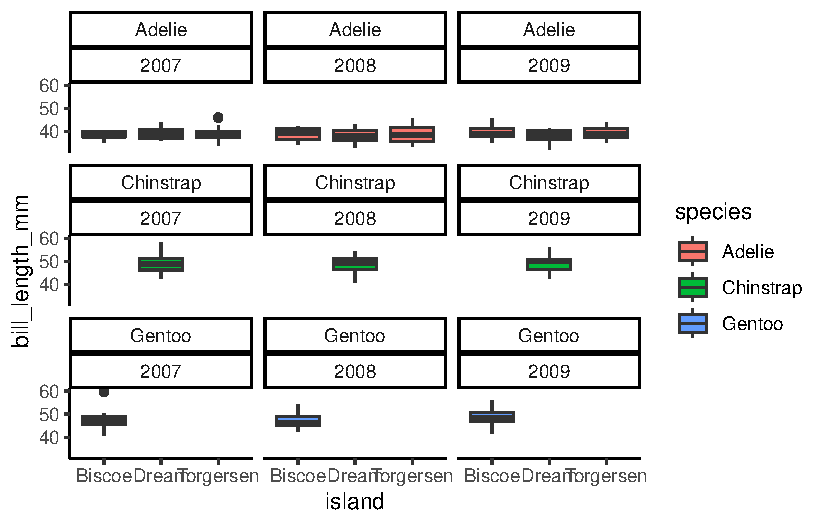
\includegraphics{facets_files/figure-pdf/unnamed-chunk-5-1.pdf}

}

\end{figure}

\begin{center}\rule{0.5\linewidth}{0.5pt}\end{center}

\hypertarget{multiple-plots-on-the-same-page}{%
\subsection{\texorpdfstring{\textbf{Multiple plots on the same
page}}{Multiple plots on the same page}}\label{multiple-plots-on-the-same-page}}

Using the simple and wonderful patchwork package, we can place multiple
plots on the same page. To do this, we must actually name each plot.
Here's an example.

Patchwork is super easy! Learn more
\href{https://patchwork.data-imaginist.com/articles/patchwork.html}{here}(with
examples)

First, let's make some graphs and name them

\begin{Shaded}
\begin{Highlighting}[]
\CommentTok{\#First, we need to calculate a mean bill length for our penguins by species and island}
\NormalTok{sumpens}\OtherTok{\textless{}{-}}\NormalTok{ penguins }\SpecialCharTok{\%\textgreater{}\%}
  \FunctionTok{group\_by}\NormalTok{(species, island) }\SpecialCharTok{\%\textgreater{}\%}
  \FunctionTok{na.omit}\NormalTok{() }\SpecialCharTok{\%\textgreater{}\%} \CommentTok{\#removes rows with NA values (a few rows may otherwise have NA due to sampling error in the field)}
  \FunctionTok{summarize}\NormalTok{(}\AttributeTok{meanbill=}\FunctionTok{mean}\NormalTok{(bill\_length\_mm), }\AttributeTok{sd=}\FunctionTok{sd}\NormalTok{(bill\_length\_mm), }\AttributeTok{n=}\FunctionTok{n}\NormalTok{(), }\AttributeTok{se=}\NormalTok{sd}\SpecialCharTok{/}\FunctionTok{sqrt}\NormalTok{(n))}
\end{Highlighting}
\end{Shaded}

\begin{verbatim}
`summarise()` has grouped output by 'species'. You can override using the
`.groups` argument.
\end{verbatim}

\begin{Shaded}
\begin{Highlighting}[]
\NormalTok{sumpens}
\end{Highlighting}
\end{Shaded}

\begin{verbatim}
# A tibble: 5 x 6
# Groups:   species [3]
  species   island    meanbill    sd     n    se
  <fct>     <fct>        <dbl> <dbl> <int> <dbl>
1 Adelie    Biscoe        39.0  2.48    44 0.374
2 Adelie    Dream         38.5  2.48    55 0.335
3 Adelie    Torgersen     39.0  3.03    47 0.442
4 Chinstrap Dream         48.8  3.34    68 0.405
5 Gentoo    Biscoe        47.6  3.11   119 0.285
\end{verbatim}

\begin{Shaded}
\begin{Highlighting}[]
\CommentTok{\# Next, we can make our graphs!}

\NormalTok{p1}\OtherTok{\textless{}{-}}\FunctionTok{ggplot}\NormalTok{(}\AttributeTok{data=}\NormalTok{penguins, }\FunctionTok{aes}\NormalTok{(bill\_length\_mm))}\SpecialCharTok{+}
  \FunctionTok{geom\_histogram}\NormalTok{()}\SpecialCharTok{+}
  \FunctionTok{theme\_classic}\NormalTok{()}


\NormalTok{p2}\OtherTok{\textless{}{-}}\FunctionTok{ggplot}\NormalTok{()}\SpecialCharTok{+}
  \FunctionTok{geom\_jitter}\NormalTok{(}\AttributeTok{data=}\NormalTok{ penguins, }\FunctionTok{aes}\NormalTok{(}\AttributeTok{x=}\NormalTok{species, }\AttributeTok{y=}\NormalTok{bill\_length\_mm, }\AttributeTok{color=}\NormalTok{island), }\AttributeTok{alpha=}\FloatTok{0.5}\NormalTok{, }\AttributeTok{width=}\FloatTok{0.2}\NormalTok{)}\SpecialCharTok{+}
  \FunctionTok{geom\_point}\NormalTok{(}\AttributeTok{data=}\NormalTok{sumpens, }\FunctionTok{aes}\NormalTok{(}\AttributeTok{x=}\NormalTok{species, }\AttributeTok{y=}\NormalTok{meanbill, }\AttributeTok{color=}\NormalTok{island), }\AttributeTok{size=}\DecValTok{3}\NormalTok{)}\SpecialCharTok{+}
  \FunctionTok{geom\_errorbar}\NormalTok{(}\AttributeTok{data=}\NormalTok{sumpens, }\FunctionTok{aes}\NormalTok{(}\AttributeTok{x=}\NormalTok{species, }\AttributeTok{ymin=}\NormalTok{meanbill}\SpecialCharTok{{-}}\NormalTok{se, }\AttributeTok{ymax=}\NormalTok{meanbill}\SpecialCharTok{+}\NormalTok{se), }\AttributeTok{width=}\FloatTok{0.1}\NormalTok{)}\SpecialCharTok{+}
  \FunctionTok{theme\_classic}\NormalTok{()}\SpecialCharTok{+}
  \FunctionTok{scale\_color\_aaas}\NormalTok{()}

\NormalTok{p3}\OtherTok{\textless{}{-}}\FunctionTok{ggplot}\NormalTok{(}\AttributeTok{data=}\NormalTok{penguins, }\FunctionTok{aes}\NormalTok{(island)) }\SpecialCharTok{+}
  \FunctionTok{geom\_bar}\NormalTok{(}\FunctionTok{aes}\NormalTok{(}\AttributeTok{fill=}\NormalTok{species), }\AttributeTok{position=} \FunctionTok{position\_dodge}\NormalTok{())}\SpecialCharTok{+}
  \FunctionTok{theme\_classic}\NormalTok{()}\SpecialCharTok{+}
  \FunctionTok{scale\_fill\_aaas}\NormalTok{()}
\end{Highlighting}
\end{Shaded}

Now let's patchwork them together! We make a simple formula to make a
patchwork. Addition puts everything in the same row. But we can use
division and other symbols to organize.

\begin{Shaded}
\begin{Highlighting}[]
\FunctionTok{library}\NormalTok{(patchwork)}

\NormalTok{p1}\SpecialCharTok{+}\NormalTok{p2}\SpecialCharTok{+}\NormalTok{p3}
\end{Highlighting}
\end{Shaded}

\begin{verbatim}
`stat_bin()` using `bins = 30`. Pick better value with `binwidth`.
\end{verbatim}

\begin{verbatim}
Warning: Removed 2 rows containing non-finite values (`stat_bin()`).
\end{verbatim}

\begin{verbatim}
Warning: Removed 2 rows containing missing values (`geom_point()`).
\end{verbatim}

\begin{figure}[H]

{\centering 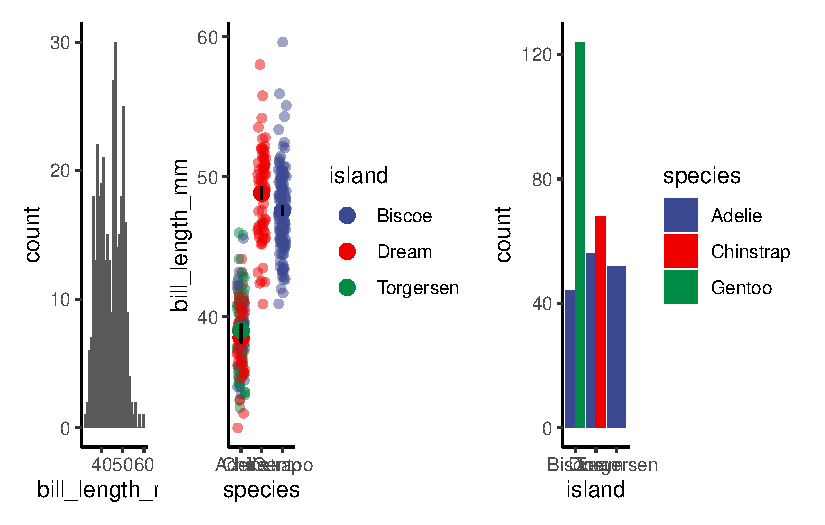
\includegraphics{facets_files/figure-pdf/unnamed-chunk-7-1.pdf}

}

\end{figure}

Division allows us to put panels in columns

\begin{Shaded}
\begin{Highlighting}[]
\NormalTok{p1}\SpecialCharTok{/}\NormalTok{p2}\SpecialCharTok{/}\NormalTok{p3}
\end{Highlighting}
\end{Shaded}

\begin{verbatim}
`stat_bin()` using `bins = 30`. Pick better value with `binwidth`.
\end{verbatim}

\begin{verbatim}
Warning: Removed 2 rows containing non-finite values (`stat_bin()`).
\end{verbatim}

\begin{verbatim}
Warning: Removed 2 rows containing missing values (`geom_point()`).
\end{verbatim}

\begin{figure}[H]

{\centering 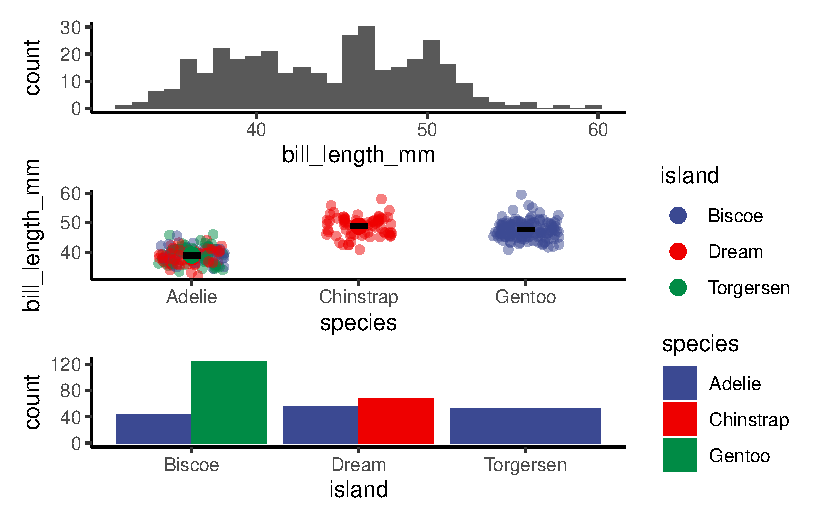
\includegraphics{facets_files/figure-pdf/unnamed-chunk-8-1.pdf}

}

\end{figure}

We can also combine addition and division (order of operations is still
a thing!)

\begin{Shaded}
\begin{Highlighting}[]
\NormalTok{(p1}\SpecialCharTok{+}\NormalTok{p2) }\SpecialCharTok{/}\NormalTok{ p3}
\end{Highlighting}
\end{Shaded}

\begin{verbatim}
`stat_bin()` using `bins = 30`. Pick better value with `binwidth`.
\end{verbatim}

\begin{verbatim}
Warning: Removed 2 rows containing non-finite values (`stat_bin()`).
\end{verbatim}

\begin{verbatim}
Warning: Removed 2 rows containing missing values (`geom_point()`).
\end{verbatim}

\begin{figure}[H]

{\centering 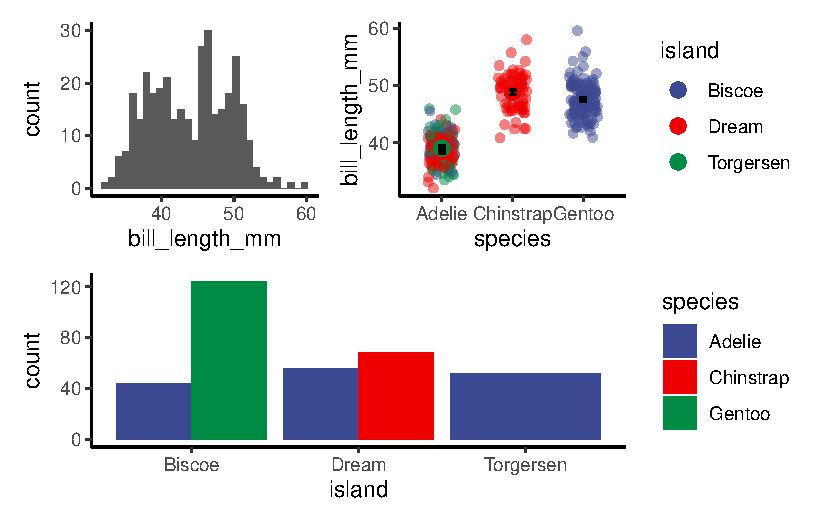
\includegraphics{facets_files/figure-pdf/unnamed-chunk-9-1.pdf}

}

\end{figure}

There are other functions in patchwork that allow us to annotate plots,
give them labels, move/combine legends, etc.

\begin{center}\rule{0.5\linewidth}{0.5pt}\end{center}



\end{document}
